\documentclass{jlreq}
\usepackage[dvipdfmx]{graphicx}
\usepackage{amsmath}
\usepackage{geometry}
\usepackage{float}
\usepackage{caption}
\usepackage{hyperref}
\usepackage[dvipdfmx,table]{xcolor}
\linespread{1.2}
\numberwithin{equation}{section}
\counterwithin{figure}{section}
\counterwithin{table}{section}

\begin{document}

\section{目的}
オペアンプ回路の製作と製作した回路の電気的特性を計測することにより、電気電子情報通信実験で使用する各種機器の基本的な扱い方と報告書の作成方法を習得する。

\section{原理}
\subsection{製作する回路}

\begin{figure}[h]
  \centering
  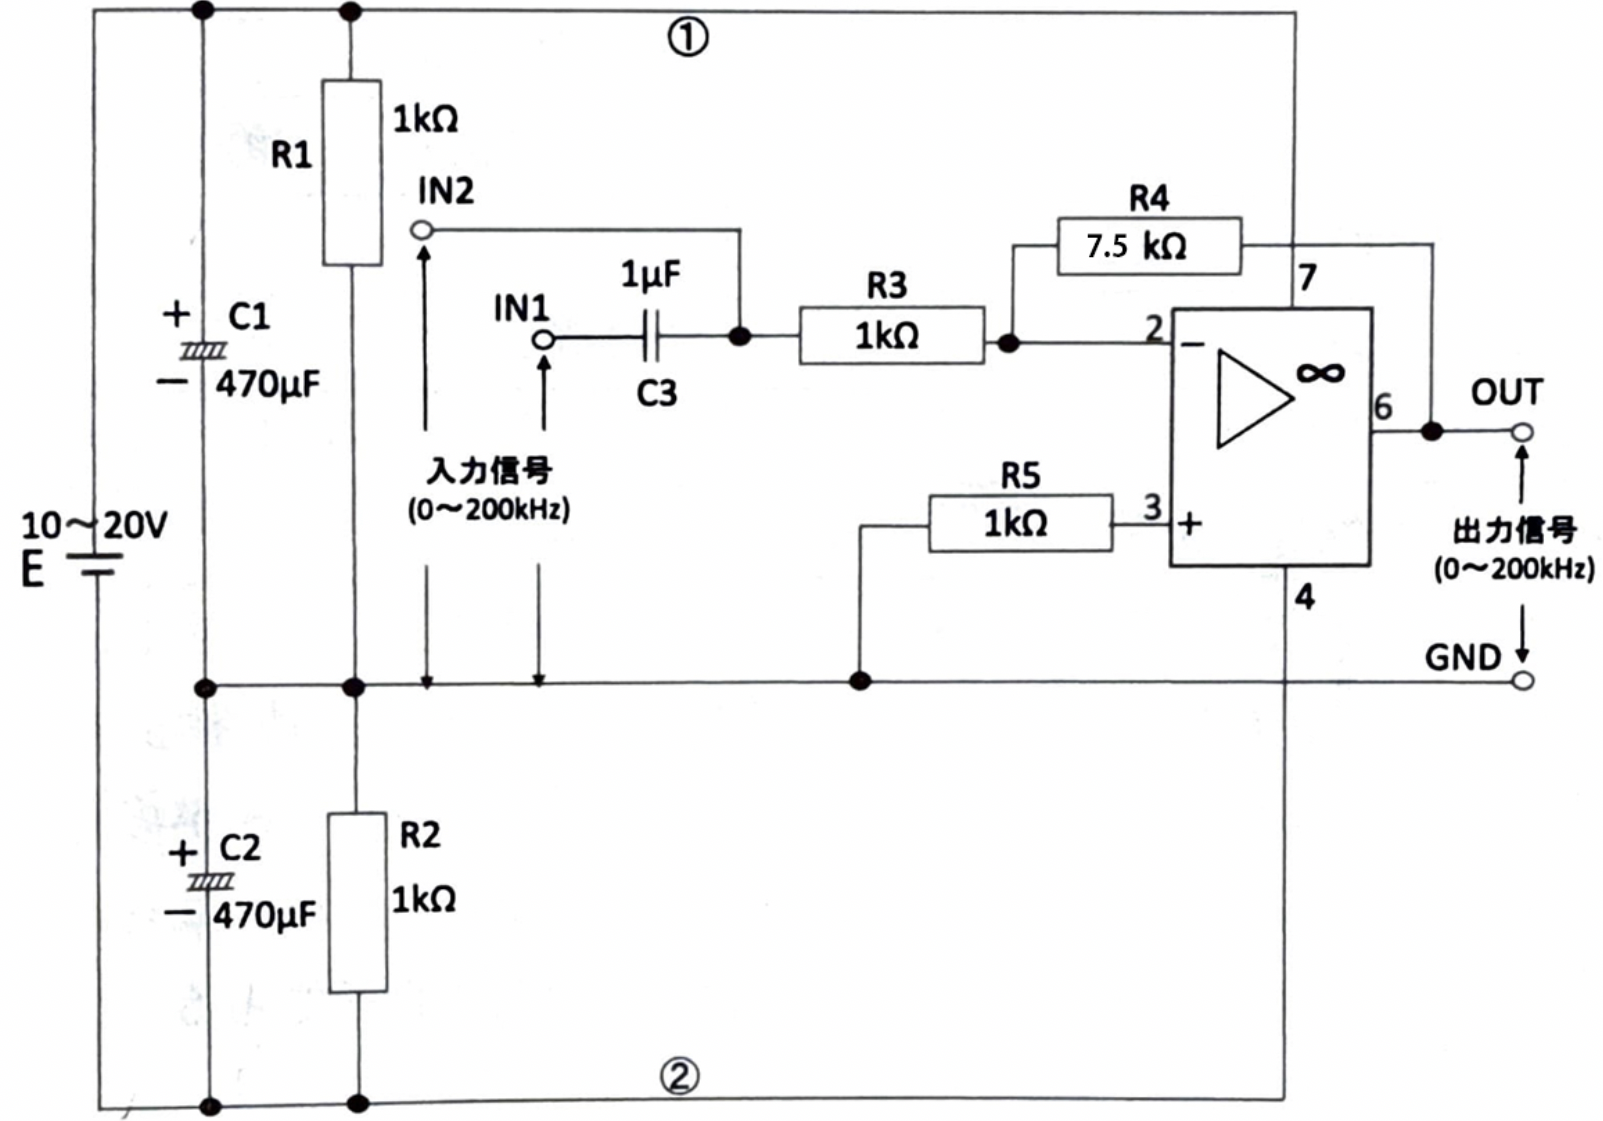
\includegraphics[width=100mm]{kairozu.png}
  \caption{オペアンプの回路}
\end{figure}

\subsection{回路の動作原理}
図4-1は、非反転入力端子\(V_+\)が接地されていることから、プラス電源のみで動作する簡単な反転増幅回路である。抵抗\(R_1\)と\(R_2\)で供給される電圧\(E_2\)を分割してOPアンプの7番ピンと4番ピンに供給している。コンデンサ\(C_1\)と\(C_2\)は電源ラインのノイズを除去し、電源電圧を一定に保つために付加している。カップリングコンデンサ\(C_3\)は直流をカットするために付加したものである。また、抵抗\(R_3\)〜\(R_5\)で反転増幅回路を構成している。

\subsection{OPアンプの7番端子と4番端子にかかる電圧}
抵抗\(R_1\)と\(R_2\)は直列に接続されており、どちらも抵抗値が10k\(\Omega\)であるため、それぞれに電源電圧\(E\)の半分、すなわち\(\frac{E}{2}\)ずつの電圧がかかる。また、\(R_1\)と\(R_2\)の接続点を接地しているため、OPアンプの7番端子には\(+\frac{E}{2}\)、4番端子には\(-\frac{E}{2}\)の電圧がかかる。

\subsection{本回路における入出力特性の理論式の導出}
オペアンプは、入力インピーダンスが高いため反転入力端子\(-\)側に電流は流れない。したがって、抵抗\(R_3\)と\(R_4\)に流れる電流は等しいと考えられる。この電流を\(I\)とすると、次の関係が成り立つ。
\begin{equation}
  I = \frac{V_\text{in} - V_-}{R_3} = \frac{V_- - V_\text{out}}{R_4}
\end{equation}

ここで、理想的なオペアンプの特性として、反転入力端子\(-\)と非反転入力端子\(+\)の電位は等しいため、\(V_- = V_+\)が成り立つ。また、非反転入力端子\(+\)は接地されているため、\(V_+ = 0\)となる。したがって、\(V_- = 0\)である。

この結果を上式に代入すると、
\begin{equation}
  I = \frac{V_\text{in}}{R_3} = \frac{-V_\text{out}}{R_4}
\end{equation}

これを整理して、出力電圧\(V_\text{out}\)を求めると、
\begin{equation}
  V_\text{out} = -\frac{R_4}{R_3}V_\text{in}
\end{equation}

したがって、本回路の入出力特性は上記のように表される。

\subsection{周波数特性の理論値の算出}
入力端子\(\text{IN}_1\)および\(\text{IN}_2\)の増幅率の周波数特性を理論的に算出する。まず、\(\text{IN}_1\)について考える。カップリングコンデンサ\(C_3\)が付加されているため、回路の周波数特性は次のように表される。

\begin{equation}
  V_\text{out} = \frac{R_4}{R_3 + \frac{1}{j\omega C_3}} V_\text{in}
\end{equation}

ここで、低周波数領域ではカップリングコンデンサ\(C_3\)の影響により増幅率が低下する。一方、高周波数領域ではコンデンサの影響が無視できるため、増幅率は一定値に近づく。

次に、\(\text{IN}_2\)について考える。\(\text{IN}_2\)には特にコンデンサが付加されていないため、周波数特性は一定であり、次のように表される。

\begin{equation}
  A_{\text{IN}_2}(f) = \left| -\frac{R_4}{R_3} \right|
\end{equation}

したがって、\(\text{IN}_1\)と\(\text{IN}_2\)の周波数特性は上記のように理論的に求められる。ここで、電圧利得を明確に計算すると、\(\text{IN}_1\)の利得は次のように表される。
まず、\(\text{IN}_1\)の周波数特性を考える。カップリングコンデンサ\(C_3\)が付加されているため、回路のインピーダンスは次のように表される。
\begin{equation}
  Z = R_3 + \frac{1}{j\omega C_3}
\end{equation}

ここで、\(\omega = 2\pi f\)は角周波数である。このインピーダンスを用いて、増幅率は次のように表される。
\begin{equation}
  A_{\text{IN}_1}(f) = \left| -\frac{R_4}{Z} \right| = \left| -\frac{R_4}{R_3 + \frac{1}{j\omega C_3}} \right|
\end{equation}

複素数の計算を簡単にするため、分母を有理化する。分母に\((R_3 - \frac{1}{j\omega C_3})\)を掛けると、
\begin{equation}
  A_{\text{IN}_1}(f) = \left| -\frac{R_4 (R_3 - \frac{1}{j\omega C_3})}{R_3^2 + \left(\frac{1}{\omega C_3}\right)^2} \right|
\end{equation}

分子の虚部はゼロになるため、絶対値を取ると次のようになる。
\begin{equation}
  A_{\text{IN}_1}(f) = \frac{R_4}{\sqrt{R_3^2 + \left(\frac{1}{2\pi f C_3}\right)^2}}
\end{equation}

これをデシベル(dB)表記に変換すると、
\begin{equation}
  A_{\text{IN}_1}(f) = 20 \log_{10} \left| \frac{R_4}{\sqrt{R_3^2 + \left(\frac{1}{2\pi f C_3}\right)^2}} \right| \, \text{[dB]}
\end{equation}

したがって、\(\text{IN}_1\)の利得は上記のように表される。

また、\(\text{IN}_2\)の利得は周波数に依存せず、次のように一定である。
\begin{equation}
  A_{\text{IN}_2}(f) = 20 \log_{10} \left| \frac{R_4}{R_3} \right| \, \text{[dB]}
\end{equation}

\subsection{電圧特性の算出値(理論値)}
式 (2.9) を用いて、入力電圧と出力電圧の関係を求める。今回、\(R_4 = 7.5\text{k}\Omega\)、\(R_3 = 1\text{k}\Omega\)、\(C_3 = 1\mu\text{F}\)、\(f = 50\text{Hz}\) であるから、\(A_{\text{IN}_1} \approx 2.24\) として理論値を計算する。

\begin{table}[H]
  \centering
  \caption{IN1 の電圧特性の理論値}
  \begin{tabular}{|c|c|}
    \hline
    入力電圧 [mVpp] & 出力電圧 [mVpp] \\ \hline
    400 & 896 \\ \hline
    500 & 1120 \\ \hline
    600 & 1344 \\ \hline
    700 & 1568 \\ \hline
    800 & 1792 \\ \hline
    900 & 2016 \\ \hline
    1000 & 2240 \\ \hline
  \end{tabular}
\end{table}

\begin{table}[H]
  \centering
  \caption{IN2 の電圧特性の理論値}
  \begin{tabular}{|c|c|}
    \hline
    入力電圧 [mVpp] & 出力電圧 [mVpp] \\ \hline
    400 & 3000 \\ \hline
    500 & 3750 \\ \hline
    600 & 4500 \\ \hline
    700 & 5250 \\ \hline
    800 & 6000 \\ \hline
    900 & 6750 \\ \hline
    1000 & 7500 \\ \hline
  \end{tabular}
\end{table}

\subsection{電圧増幅率の算出値(理論値)}
式 (2.5) と (2.9) を用いて、IN1とIN2の電圧増幅率を求める。今回、\(R_4 = 7.5\text{k}\Omega\)、\(R_3 = 1\text{k}\Omega\)、\(C_3 = 1\mu\text{F}\)であるから、次のように計算する。

IN1の電圧増幅率については、
\begin{equation}
  A_{\text{IN}_1}(f) = \frac{R_4}{\sqrt{R_3^2 + \left(\frac{1}{2\pi f C_3}\right)^2}} = \frac{7.5k\Omega}{\sqrt{(1k\Omega)^2 + \left(\frac{1}{2\pi f \cdot 1\mu\text{F}}\right)^2}}
\end{equation}

IN2の電圧増幅率については、
\begin{equation}
  A_{\text{IN}_2} = \frac{R_4}{R_3} = \frac{7.5k\Omega}{1k\Omega} = 7.5
\end{equation}
このように計算できる。

\subsection{低域側と高域側の違いについて}
本回路における低域側と高域側の違いは、主にカップリングコンデンサ\(C_3\)の影響によるものである。

低域側では、カップリングコンデンサ\(C_3\)のインピーダンスが高くなるため、入力信号が減衰しやすい。この結果、回路全体の増幅率が低下する。具体的には、カップリングコンデンサのインピーダンスは次式で表される。
\[
Z_{C_3} = \frac{1}{j\omega C_3}
\]
ここで、角周波数\(\omega = 2\pi f\)が小さい(低周波数)場合、\(Z_{C_3}\)が大きくなり、信号がコンデンサを通過しにくくなるため、増幅率が低下する。

一方、高域側では、カップリングコンデンサ\(C_3\)のインピーダンスが低くなるため、入力信号がほぼそのまま回路に伝達される。この結果、回路の増幅率は抵抗比\(-\frac{R_4}{R_3}\)に近づき、一定値を示す。

したがって、低域側ではカップリングコンデンサの影響により増幅率が低下し、高域側ではその影響が無視できるため、増幅率が一定となると理論的に考えられる。

\section{実験方法}
\subsection{使用機材}
\begin{itemize}
  \item ハンダゴテ
  \item 直流安定化電源
  \item デジタル・マルチメーター(テスター)
  \item 信号発生装置
  \item デジタル・オシロスコープ
\end{itemize}

\subsection{使用する部品一覧}
\begin{table}[H]
  \centering
  \caption{使用する部品一覧}
  \begin{tabular}{|c|l|c|l|}
    \hline
    項番 & 品名 & 数量 & 備考 \\ \hline
    1 & ユニバーサル基板 & 1 & 95×72mm \\ \hline
    2 & 汎用オペアンプ & 1 & LM741 または NJM741 \\ \hline
    3 & 金属皮膜抵抗器 (7.5k\(\Omega\), 1/4W) & 1 & \\ \hline
    4 & 金属皮膜抵抗器 (1k\(\Omega\), 1/4W) & 4 & \\ \hline
    5 & 電解コンデンサ (470\(\mu\)F, 16V) & 2 & \\ \hline
    6 & 積層セラミックコンデンサ (1\(\mu\)F, 50V) & 1 & \\ \hline
  \end{tabular}
\end{table}
この他に、ハンダ付けするための線材(スズメッキ線)とハンダが必要である。

\subsection{回路の組み立て}
\begin{enumerate}
  \item 部品配置を検討する。
    \begin{itemize}
      \item 電源端子の位置を考慮し、電源供給が容易な配置にする。
      \item GND端子は、信号発生器やデジタル・オシロスコープなど複数の機器が接続しやすいようにする。
      \item 信号入力端子(IN1, IN2)を適切に配置し、信号発生器とデジタル・オシロスコープが接続しやすいようにする。また、GND端子と対になるように配置する。
    \end{itemize}
  \item 配線方法を検討する。
    \begin{itemize}
      \item 配線は極力直線的にし、交差や無駄を避ける。スズメッキ線は極力直線、直角にすることで判別しやすくする。
      \item 部品の配置を基板の銅箔面(実装面)に合わせて行い、効率的な配線を目指す。
      \item OPアンプのピン配置を確認し、誤接続を防ぐ。データシートのピン配置図を参考にし、特にTop viewとBottom viewの違いに注意する。
      \item 配線が交差する際は、基板の裏面を利用して交差させる。
    \end{itemize}
\end{enumerate}

\subsection{回路の接続と測定手順}
ファンクションジェネレーターとオシロスコープのCH1を、それぞれ製作した回路のIN1端子(もしくはIN2端子)とGND端子間に繋ぐ。これにより、ファンクションジェネレーターの出力電圧は、オシロスコープでのCH1の測定値をもとに調整する。次に、オシロスコープのCH2をOUT端子とGND端子間に繋ぎ、出力電圧を測定する。これにより、IN1端子(もしくはIN2端子)からの入力信号に対する出力信号の変化を観測することができる。

\subsection{実験課題}
\subsubsection{電圧特性の測定}
\begin{enumerate}
  \item 入力信号を50Hzで\(\text{IN}_1\)と\(\text{IN}_2\)に入力し、出力信号の電圧の振幅(ピークピーク値)をデジタル・オシロスコープで測定する。
  \item 入力電圧を400mVpp, 500mVpp, 600mVpp, 700mVpp, 800mVpp, 900mVpp, 1Vppに設定し、入力電圧と出力電圧の関係をグラフで表す。
  \item 作成したOPアンプ回路の理論値を算出し、測定結果との相違について考察する。
\end{enumerate}

\subsubsection{周波数特性の測定}
\begin{enumerate}
  \item 入力信号の電圧振幅を一定(500mV)にし、周波数を5~200kHzまで変化させたときの出力電圧をデジタル・オシロスコープで測定する。
  \item 入力周波数と出力電圧の関係をグラフで表す。
  \item 作成したOPアンプ回路の理論値を算出し、測定結果との相違について考察する。
\end{enumerate}

\subsubsection{リサージュ図形の測定}
\begin{enumerate}
  \item 入力信号をデジタル・オシロスコープのチャンネル1、出力信号をチャンネル2に入力し、入力信号の周波数を500Hz~10kHzまで変化させたときのリサージュ図形を確認する。
  \item 代表的なリサージュ図形をスケッチし、理論値との違いについて考察する。
\end{enumerate}

\subsubsection{デジタル・オシロスコープの操作}
\begin{enumerate}
  \item 1kHzのサイン補正信号をCH1のプローブに入力し、FFT表示させて波形をグラフ用紙に記録する。
  \item FFT表示の第1~第3高調波の周波数を読み取り、矩形波を表すフーリエ級数の式との関係について考察する。
\end{enumerate}

\section{実験結果}

\subsection{各部の電圧測定}
製作した回路の各部の電圧を測定した。測定結果は表4.1の通りである。
\begin{table}[H]
  \centering
  \caption{各部の電圧測定結果}
  \begin{tabular}{|c|c|c|c|c|c|}
    \hline
    測定部位 & 1-2間 & GND-1間 & GND-2間 & GND-OPアンプの7番ピン間 & GND-OPアンプの4番ピン間 \\ \hline
    電圧[V] & 15.8 & 7.8 & -7.8 & 7.8 & -7.8\\ \hline
  \end{tabular}
\end{table}

\subsection{電圧特性の測定}
入力周波数を50Hzで一定にし、入力電圧の振幅を400mVpp〜1000mVppまで変化させたときの出力電圧をデジタル・オシロスコープで測定した。入力電圧は、信号発生器からの出力をデジタル・オシロスコープで測定し、出力電圧は、OPアンプの出力端子からの信号をデジタル・オシロスコープで測定した。
IN1,IN2それぞれの計測結果は表4.2,表4.3の通りである。またこれらのグラフを図4.1に示す。グラフは、横軸に入力電圧、縦軸に出力電圧を取ったものである。

\begin{table}[H]
  \centering
  \caption{IN1 の電圧特性の理論値と測定結果}
  \begin{tabular}{|c|c|c|c|c|}
    \hline
      \color{blue}{入力電圧(理論値) [mVpp]} & \color{blue}{出力電圧(理論値) [mVpp]} & \color{blue}{入力電圧(実測値) [mVpp]} & \color{blue}{出力電圧(実測値) [mVpp]} \\ \hline
      \color{blue}{400} & \color{blue}{896} & \color{blue}{408} & \color{blue}{900} \\ \hline
      \color{blue}{500} & \color{blue}{1120} & \color{blue}{500} & \color{blue}{1120} \\ \hline
      \color{blue}{600} & \color{blue}{1344} & \color{blue}{600} & \color{blue}{1320} \\ \hline
      \color{blue}{700} & \color{blue}{1568} & \color{blue}{700} & \color{blue}{1600} \\ \hline
      \color{blue}{800} & \color{blue}{1792} & \color{blue}{800} & \color{blue}{1920} \\ \hline
      \color{blue}{900} & \color{blue}{2016} & \color{blue}{920} & \color{blue}{2160} \\ \hline
      \color{blue}{1000} & \color{blue}{2240} & \color{blue}{1060} & \color{blue}{2480} \\ \hline
  \end{tabular}
\end{table}

\begin{table}[H]
  \centering
  \caption{IN2 の電圧特性の理論値と測定結果}
  \begin{tabular}{|c|c|c|c|}
    \hline
      \color{blue}{入力電圧(理論値)} [mVpp] & \color{blue}{出力電圧(理論値) [mVpp]} & \color{blue}{入力電圧(実測値) [mVpp]} & \color{blue}{出力電圧(実測値) [mVpp]} \\ \hline
      \color{blue}{400} & \color{blue}{3000} & \color{blue}{404} & \color{blue}{2860} \\ \hline
      \color{blue}{500} & \color{blue}{3750} & \color{blue}{504} & \color{blue}{3640} \\ \hline
      \color{blue}{600} & \color{blue}{4500} & \color{blue}{604} & \color{blue}{4380} \\ \hline
      \color{blue}{700} & \color{blue}{5250} & \color{blue}{704} & \color{blue}{5080} \\ \hline
      \color{blue}{800} & \color{blue}{6000} & \color{blue}{800} & \color{blue}{5920} \\ \hline
      \color{blue}{900} & \color{blue}{6750} & \color{blue}{900} & \color{blue}{6640} \\ \hline
      \color{blue}{1000} & \color{blue}{7500} & \color{blue}{1020} & \color{blue}{7460} \\ \hline
  \end{tabular}
\end{table}

\subsection{周波数特性の測定}
入力電圧の振幅を500mVで一定にし、入力周波数を5〜200kHzまで変化させたときの出力電圧を測定した。IN1,IN2それぞれの計測結果は表4.4,表4.5の通りである。またこれらのグラフを図4.2示す。グラフは、横軸に入力周波数、縦軸に出力電圧を取ったものである。

\begin{table}[H]
  \centering
  \caption{IN1 の周波数特性の理論値と測定結果}
  \begin{tabular}{|c|c|c|}
    \hline
    周波数 [Hz] & 出力電圧 [mVpp] (理論値) & 出力電圧 [mVpp] (実測値) \\ \hline
    5 & 117 & 160 \\ \hline
    10 & 235 & 320 \\ \hline
    20 & 467 & 480 \\ \hline
    30 & 694 & 720 \\ \hline
    40 & 914 & 960 \\ \hline
    50 & 1123 & 1120 \\ \hline
    60 & 1322 & 1360 \\ \hline
    70 & 1509 & 1440 \\ \hline
    80 & 1684 & 1600 \\ \hline
    90 & 1845 & 1760 \\ \hline
    100 & 1995 & 1920 \\ \hline
    200 & 2934 & 2720 \\ \hline
    500 & 3573 & 3280 \\ \hline
    1000 & 3703 & 3440 \\ \hline
    2000 & 3738 & 3520 \\ \hline
    5000 & 3748 & 3520 \\ \hline
    10000 & 3750 & 3520 \\ \hline
    20000 & 3750 & 3750 \\ \hline
    50000 & 3750 & 3600 \\ \hline
    100000 & 3750 & 2960 \\ \hline
    200000 & 3750 & 1800 \\ \hline
  \end{tabular}
\end{table}

\begin{table}[H]
  \centering
  \caption{IN2 の周波数特性の理論値と測定結果}
  \begin{tabular}{|c|c|c|}
    \hline
    周波数 [Hz] & 出力電圧 [mVpp] (理論値) & 出力電圧 [mVpp] (実測値) \\ \hline
    5 & 3750 & 4000 \\ \hline
    10 & 3750 & 4000\\ \hline
    20 & 3750 & 4000 \\ \hline
    30 & 3750 & 4000 \\ \hline
    40 & 3750 & 4000 \\ \hline
    50 & 3750 & 4000 \\ \hline
    60 & 3750 & 4000 \\ \hline
    70 & 3750 & 4000 \\ \hline
    80 & 3750 & 4000 \\ \hline
    90 & 3750 & 4000 \\ \hline
    100 & 3750 & 4000 \\ \hline
    200 & 3750 & 4000 \\ \hline
    500 & 3750 & 4000 \\ \hline
    1000 & 3750 & 4000 \\ \hline
    2000 & 3750 & 4000 \\ \hline
    5000 & 3750 & 4000 \\ \hline
    10000 & 3750 & 4000 \\ \hline
    20000 & 3750 & 4000 \\ \hline
    50000 & 3750 & 4000 \\ \hline
    100000 & 3750 & 3200 \\ \hline
    200000 & 3750 & 2000 \\ \hline
  \end{tabular}
\end{table}

\stepcounter{figure}
\stepcounter{figure}

\subsection{リサージュ図形の測定}
\subsubsection{IN1のリサージュ図形}

\begin{figure}[H]
  \centering
  \begin{minipage}{0.45\textwidth}
    \centering
    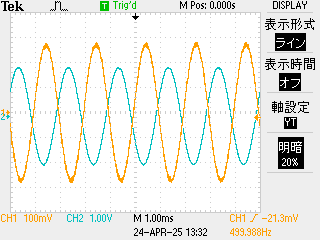
\includegraphics[width=\textwidth, keepaspectratio]{IN1_500Hz_YT.png}
    \caption{IN1の入力信号(500Hz)}
  \end{minipage}
  \hfill
  \begin{minipage}{0.45\textwidth}
    \centering
    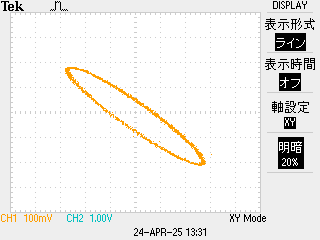
\includegraphics[width=\textwidth, keepaspectratio]{IN1_500Hz_XY.png}
    \caption{IN1のリサージュ図形(500Hz)}
  \end{minipage}
\end{figure}

\begin{figure}[H]
  \centering
  \begin{minipage}{0.45\textwidth}
    \centering
    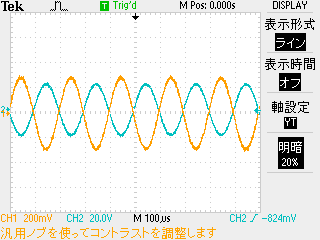
\includegraphics[width=\textwidth, keepaspectratio]{IN1_5kHz_YT.png}
    \caption{IN1の入力信号(5kHz)}
  \end{minipage}
  \hfill
  \begin{minipage}{0.45\textwidth}
    \centering
    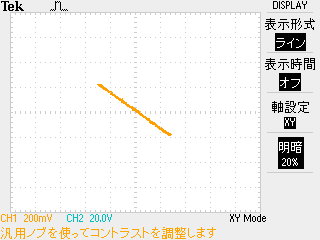
\includegraphics[width=\textwidth, keepaspectratio]{IN1_5kHz_XY.png}
    \caption{IN1のリサージュ図形(5kHz)}
  \end{minipage}
\end{figure}

500Hzと5kHzで計測したところ、図4.3から図4.6が観察できた。
500Hzでは、リサージュ図形が楕円形であることから、位相がずれていることがわかる。一方、5kHzでは直線に近い形状をしているため、逆位相になっていることが確認できる。

\subsubsection{IN2のリサージュ図形}
\begin{figure}[H]
  \centering
  \begin{minipage}{0.45\textwidth}
    \centering
    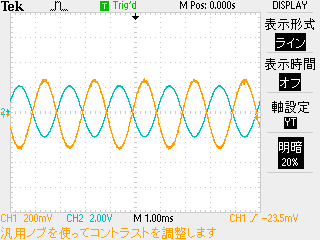
\includegraphics[width=\textwidth, keepaspectratio]{IN2_500Hz_YT.png}
    \caption{IN2の入力信号(500Hz)}
  \end{minipage}
  \hfill
  \begin{minipage}{0.45\textwidth}
    \centering
    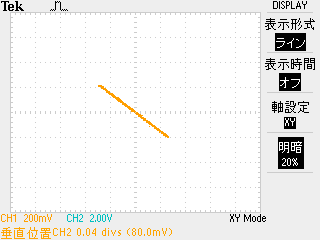
\includegraphics[width=\textwidth, keepaspectratio]{IN2_500Hz_XY.png}
    \caption{IN2のリサージュ図形(500Hz)}
  \end{minipage}
\end{figure}

\begin{figure}[H]
  \centering
  \begin{minipage}{0.45\textwidth}
    \centering
    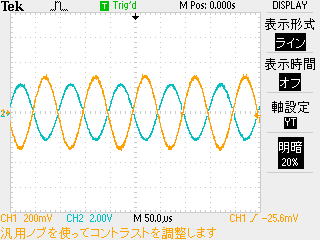
\includegraphics[width=\textwidth, keepaspectratio]{IN2_10kHz_YT.png}
    \caption{IN2の入力信号(10kHz)}
  \end{minipage}
  \hfill
  \begin{minipage}{0.45\textwidth}
    \centering
    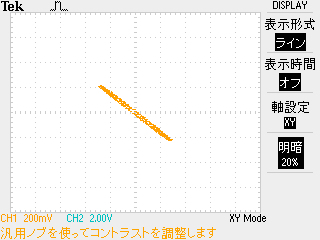
\includegraphics[width=\textwidth, keepaspectratio]{IN2_10kHz_XY.png}
    \caption{IN2のリサージュ図形(10kHz)}
  \end{minipage}
\end{figure}

500Hzと10kHzで計測したところ、図4.7から図4.10が観察された。他の周波数でも同様の傾向が見られ、リサージュ図形が直線に近い形状をしていることから、遅れなく逆位相になっていることが確認できた。

\subsubsection{100kHzのリサージュ図形}
\begin{figure}[H]
  \centering
  \begin{minipage}{0.45\textwidth}
    \centering
    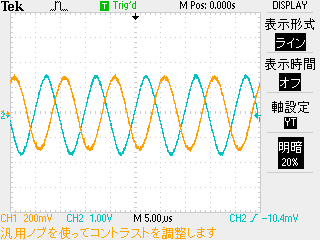
\includegraphics[width=\textwidth, keepaspectratio]{IN1_100kHz_YT.png}
    \caption{IN1の入力信号(100kHz)}
  \end{minipage}
  \hfill
  \begin{minipage}{0.45\textwidth}
    \centering
    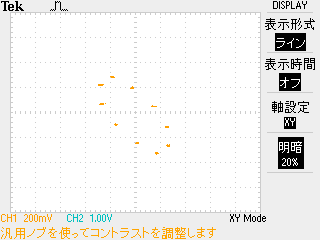
\includegraphics[width=\textwidth, keepaspectratio]{IN1_100kHz_XY.png}
    \caption{IN1のリサージュ図形(100kHz)}
  \end{minipage}
\end{figure}
\begin{figure}[H]
  \centering
  \begin{minipage}{0.45\textwidth}
    \centering
    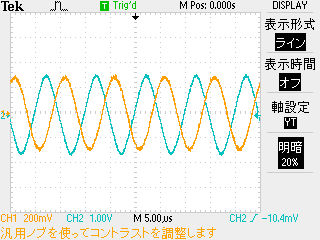
\includegraphics[width=\textwidth, keepaspectratio]{IN2_100kHz_YT.png}
    \caption{IN2の入力信号(100kHz)}
  \end{minipage}
  \hfill
  \begin{minipage}{0.45\textwidth}
    \centering
    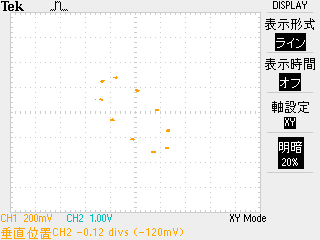
\includegraphics[width=\textwidth, keepaspectratio]{IN2_100kHz_XY.png}
    \caption{IN2のリサージュ図形(100kHz)}
  \end{minipage}
\end{figure}

100kHzでのIN1,IN2のリサージュ図形を観察したところ、図4.12,図4.14のようにどちらも楕円形のリサージュ図形が観察された。これは、位相がズレていることを示している。

\subsection{デジタル・オシロスコープの操作}

1kHzのサイン補正信号をCH1に入力し、FFT 表示させた

\begin{figure}[H]
  \centering
  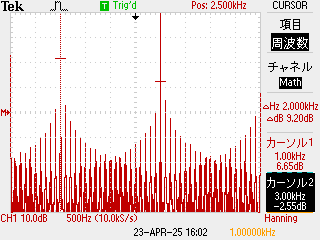
\includegraphics[width=70mm]{FFT.png}
  \caption{FFT表示}
\end{figure}

図4.15より、1kHz、3kHz、5kHzで信号が大きくなっていることがわかる。

\subsection{クリッピングの観察(任意課題)}
IN2において直流電源を6V、入力周波数を50Hzとし、電圧特性を観察した。ファンクションジェネレーターの出力電圧が350mVpp程度まではクリッピング現象は確認されなかったが、それ以上の電圧ではクリッピングが発生した。その際のオシロスコープの表示を図4.16および図4.17に示す。また、クリッピング現象が顕著に観察できる1140mVppでのオシロスコープの表示を図4.18および図4.19に示す。

\begin{figure}[H]
  \centering
  \begin{minipage}{0.45\textwidth}
    \centering
    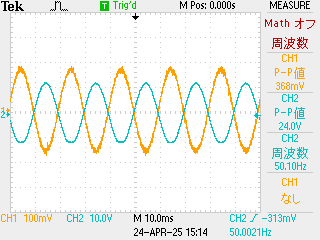
\includegraphics[width=\textwidth]{clip_350mV_YT.png}
    \caption{入力信号(50Hz 350mV)}
  \end{minipage}
  \hfill
  \begin{minipage}{0.45\textwidth}
    \centering
    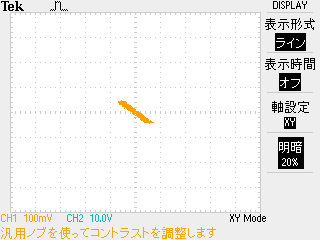
\includegraphics[width=\textwidth]{clip_350mV_XY.png}
    \caption{リサージュ図形(50Hz 350mV)}
  \end{minipage}
\end{figure}

\begin{figure}[H]
  \centering
  \begin{minipage}{0.45\textwidth}
    \centering
    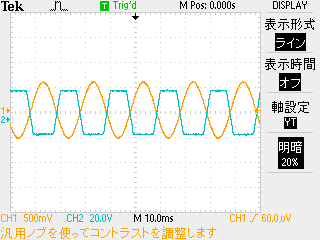
\includegraphics[width=\textwidth]{clip_1140mV_YT.png}
    \caption{入力信号(50Hz 1140mV)}
  \end{minipage}
  \hfill
  \begin{minipage}{0.45\textwidth}
    \centering
    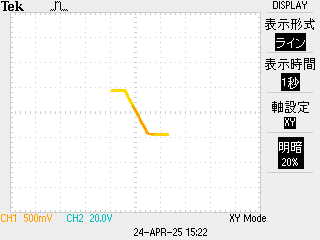
\includegraphics[width=\textwidth]{clip_1140mV_XY.png}
    \caption{リサージュ図形(50Hz 1140mV)}
  \end{minipage}
\end{figure}

\section{考察}
\subsection{各部の電圧について}
安定化電源からは16Vを出力したが、測定結果では1-2間で15.8Vとなり、0.2Vの誤差が確認された。同様に、GND-1間およびGND-2間でもそれぞれ7.8Vおよび-7.8Vと、理論値から0.2Vの誤差が生じていた。この誤差の原因としては、以下の要因が考えられる。

\begin{itemize}
  \item \textbf{測定機器の精度}: 使用したデジタル・マルチメーター(テスター)の測定精度が完全ではなく、内部の誤差が影響した可能性がある。
  \item \textbf{接触抵抗}: テスターのプローブと測定ポイントの接触が不完全であった場合、微小な電圧降下が発生した可能性がある。
  \item \textbf{電源電圧}: 安定化電源自体の出力電圧に誤差があった可能性がある。今回の誤差は一貫して0.2Vであることを踏まえると、安定化電源の出力電圧が表示上は16Vであっても、実際は15.8Vであった可能性がある。
\end{itemize}

これらの要因を踏まえると、最も有力な原因は電源装置の精度不足であると推測される。今後の実験では、より高精度な測定機器を使用するか、複数回測定して平均値を取ることで、誤差を低減することが望ましい。

\subsection{電圧特性の測定}
図2のグラフから読み取れるように、IN1およびIN2の測定値は理論値に近い結果が得られた。しかし、理論値よりも高い値や低い値が観測された箇所があり、その要因の1つとしてファンクションジェネレータの出力電圧を調整する際に、ツマミ操作が手動で行われたため正確な設定が難しく、オシロスコープでの電圧の測定値も不安定であったことが挙げられる。

\subsection{周波数特性の測定}
図19のデータシートに示されているように、オペアンプの利得は周波数が高くなるにつれて減少する。この現象は、オペアンプの利得帯域幅積(GB積)によるものである。GB積は、オペアンプの利得と周波数の積が一定であることを示しており、周波数が高くなると利得が低下することを意味する。

今回の実験では、10kHz未満の周波数では理論値に近い結果が得られたが、高周波(100kHz以上)では利得が下がる傾向が観測された。この現象を説明するために、利得は次式で計算される。
\begin{equation}
  A_v = 20 \log_{10} \left( \frac{7.5\text{k}\Omega}{10\text{k}\Omega} \right) \approx 17.5 \, \text{dB}
\end{equation}
この結果は、図5.1に示されているように、利得が周波数に応じて減少し、特に高周波では急激に低下する特性と一致している。

さらに、オペアンプのGB積が一定であることから、周波数が高くなるにつれて利得が制限されることが確認された。今回の実験では、利得が17.5dBであることが確認され、データシートのグラフにおける該当部分の周波数が約100kHzであることと一致している。このことから、実験結果はオペアンプの理論的な周波数特性を概ね正確に反映しているといえる。

また、IN2の系統誤差については、5.2節の電圧特性の測定と同様の理由によるものと考えられる。

\begin{figure}[H]
  \centering
  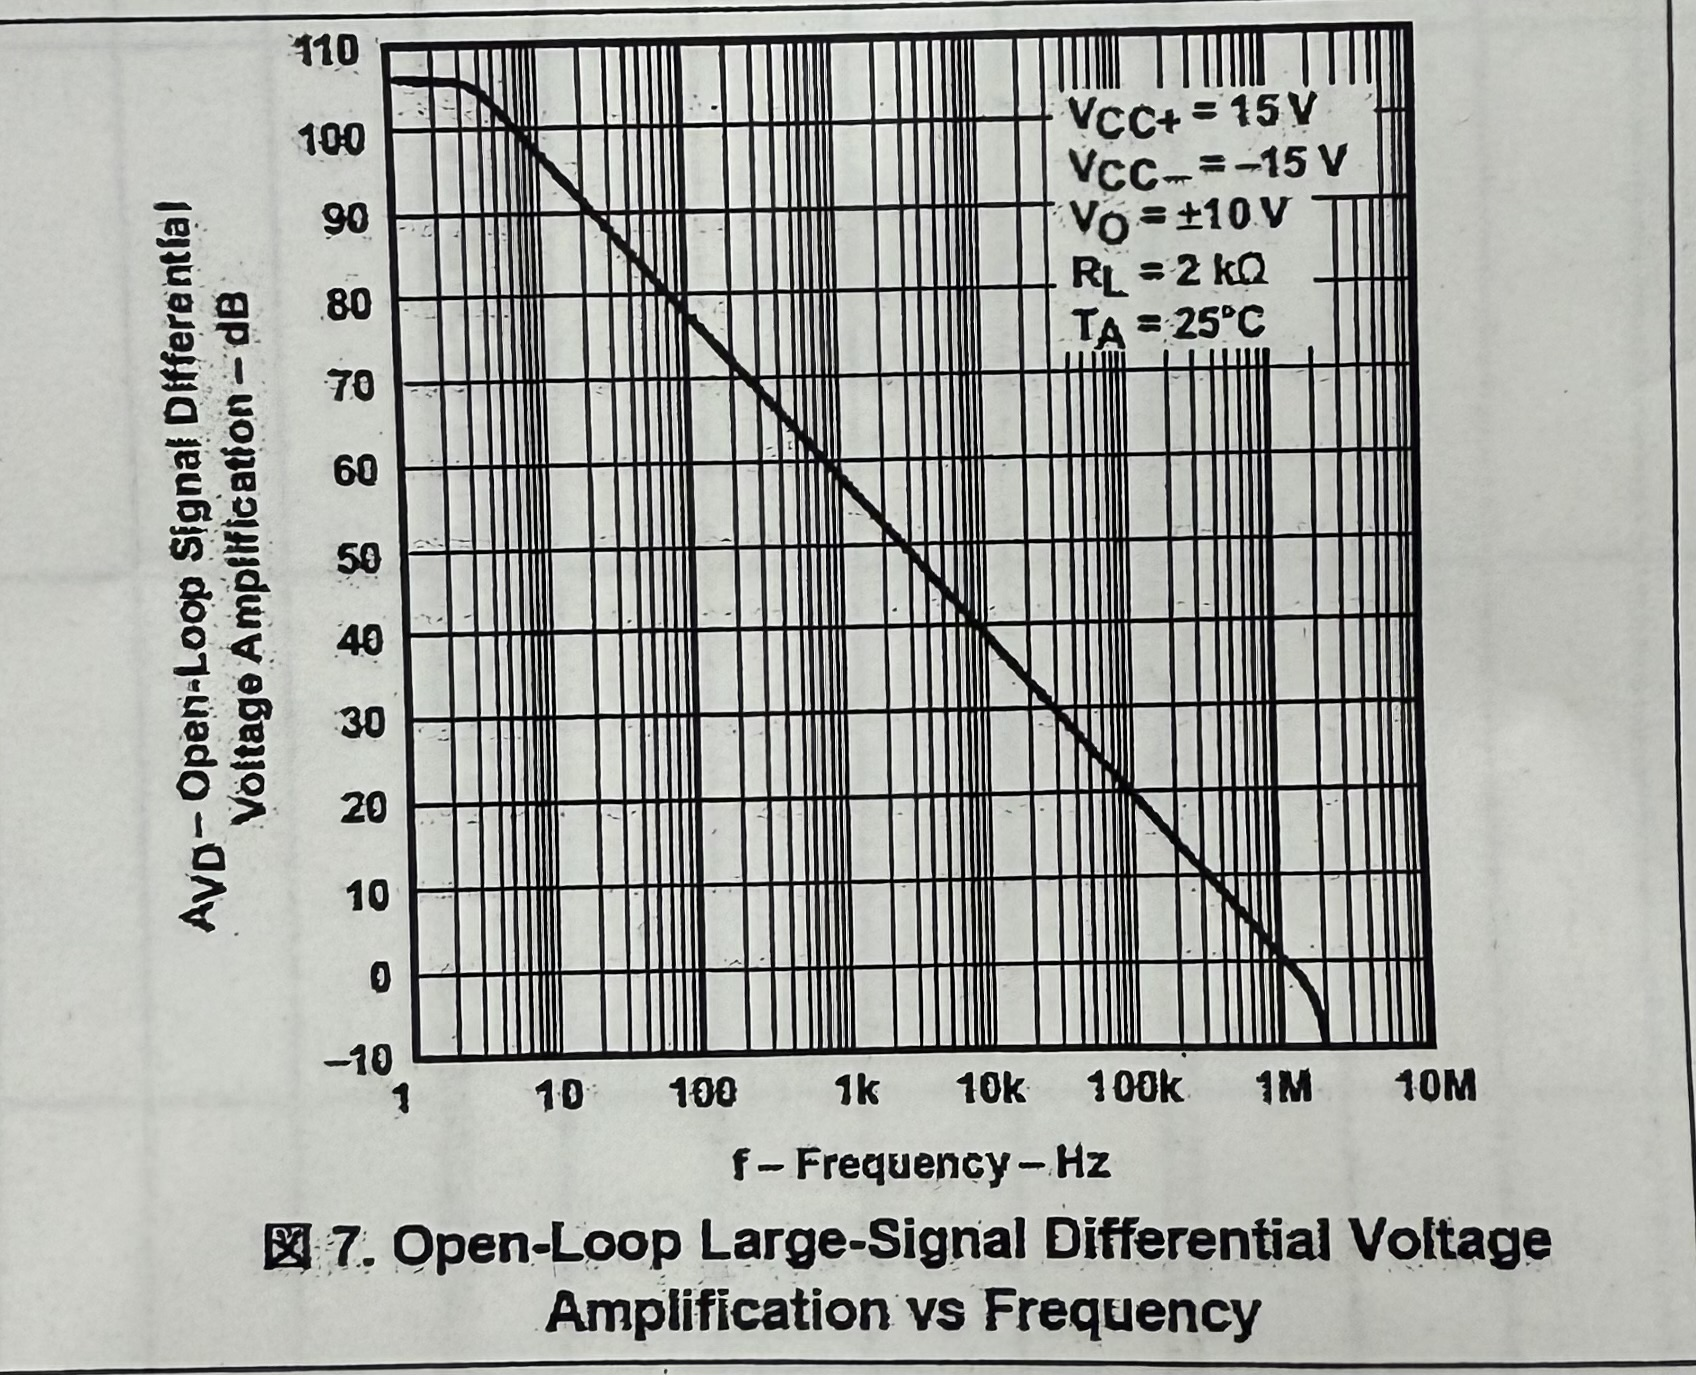
\includegraphics[width=70mm, keepaspectratio]{data.png}
  \caption{オペアンプの利得帯域幅特性(データシートより)}
\end{figure}

\subsection{リサージュ図形の測定}
\subsubsection{IN1のリサージュ図形}
500Hzでは、リサージュ図形が楕円形を示したが、これはオペアンプの反転増幅回路においてカップリングコンデンサ\(C_3\)の影響が顕著であるためである。カップリングコンデンサは低周波数領域で高いインピーダンスを持つため、入力信号の一部が減衰し、位相遅れが発生する。この位相遅れがリサージュ図形に楕円形として現れると考えられる。

一方、5kHzでは、カップリングコンデンサのインピーダンスが低下し、入力信号がほぼそのまま回路に伝達される。この結果、位相遅れがほとんどなくなり、リサージュ図形が直線に近い形状を示す。さらに、反転増幅回路の特性として、出力信号は入力信号と逆位相になるため、直線の傾きが負になることが確認できる。

したがって、低周波数ではカップリングコンデンサの影響により位相遅れが生じ、高周波数ではその影響が無視できるため、逆位相の直線が観察されると考えられる。

\subsubsection{IN2のリサージュ図形}
IN2のリサージュ図形は、500Hzでも10kHzでも同様に負の傾きを持つ直線が観察された。これは、IN2の回路にはカップリングコンデンサが存在しないため、周波数に依存した位相遅れが発生しないことによるものであると考えられる。


\subsubsection{100kHzのリサージュ図形}
100kHzでは、IN1とIN2の両方で楕円形のリサージュ図形が観察された。これは、オペアンプの高周波数領域での利得低下に伴い位相遅れが生じるためだと考えられる。また、周波数が高いということは周期が短いことを意味し、信号が回路を通過する際の遅延が相対的に大きくなるため、位相遅れが顕著になると考えられる。特に、IN1のカップリングコンデンサC3の影響が高周波では無視できることから、IN1とIN2でほぼ同様の結果が得られたとみなせる。

\subsection{サイン補正信号のFFT表示}
4.5のような結果となったのは、矩形波をフーリエ級数展開した際に特定の高調波成分が含まれるためであると考察できる。具体的には、矩形波は次式で表される。
\begin{equation}
  f(t) = \frac{4}{\pi} \left( \sin(2\pi f_0 t) + \frac{1}{3} \sin(2\pi \cdot 3 f_0 t) + \frac{1}{5} \sin(2\pi \cdot 5 f_0 t) + \frac{1}{7} \sin(2\pi \cdot 7 f_0 t) + \dots \right)
\end{equation}
ここで、\(f_0\)は基本周波数である。この式からもわかるように、矩形波は基本周波数とその奇数次高調波成分から構成されている。

したがって、FFT表示(高速フーリエ変換)においても、基本周波数の成分が最も大きく、高調波成分はその奇数倍の周波数で現れる。

\subsection{クリッピングの観察}
今回の実験で観測されたクリッピングが生じる入力電圧の閾値は、目測値で約350mVppであった。オペアンプは、供給電圧を超える出力電圧を生成することができないため、入力信号がオペアンプの供給電圧を超えると、出力信号にクリッピング現象が発生する。この現象は、オペアンプの動作範囲を超えた場合に起こり、出力信号が供給電圧に制限されることによって引き起こされる。

今回の実験では、IN2の理論上の増幅率が \(7.5\) 倍であることから、供給電圧 \(6 \, \mathrm{V}\) の場合、クリッピングの閾値は次式で計算できる。
\[
\frac{6 \, \mathrm{V}}{7.5} = 0.8 \, \mathrm{V} = 400 \, \mathrm{mV_{pp}}
\]
ここで、IN2の周波数特性測定時に記録された出力電圧が \(4000 \, \mathrm{mV_{pp}}\) であることから、この誤差を系統誤差と仮定すると、増幅率は次のように計算できる。
\[
\frac{4000 \, \mathrm{mV_{pp}}}{500 \, \mathrm{mV_{pp}}} = 8倍
\]
この場合、クリッピングの閾値は次式で計算できる。
\[
\frac{6 \, \mathrm{V}}{8} = 0.75 \, \mathrm{V} = 375 \, \mathrm{mV_{pp}}
\]

これらの計算結果は、実験で観測された \(350 \, \mathrm{mV_{pp}}\) 程度でクリッピングが発生したという目測値と概ね一致しており、実験結果が理論的な計算と整合していることが確認できた。

\subsection{使用機材}
使用機材は表10の通りである。
\begin{table}[H]
  \centering
  \caption{使用機材一覧}
  \begin{tabular}{|c|c|c|c|}
    \hline
    名称 & 型式 & 製造元 & 管理番号 \\ \hline
    直流電流源 & PMC35-1.2DU & KIKUSUI & UK002986 \\ \hline
    ファンクションジェネレータ & FG-274 & TEXIO & 17073061 \\ \hline
    オシロスコープ & TDS 2004B & Tektronix & C100578 \\ \hline
    デジタルマルチメータ & CD731 & Sanwa & 0152985 \\ \hline
  \end{tabular}
\end{table}

\subsection{参考文献}
\begin{itemize}
  \item 「オペアンプの周波数特性」, \\
  \url{https://detail-infomation.com/opamp-frequency-characteristic/}, \\
  閲覧日: 2025年4月24日
  \item 「オペアンプの基礎知識」, 日清紡マイクロデバイス株式会社, \\
  \url{https://www.nisshinbo-microdevices.co.jp/ja/design-support/basic-opamp/}, \\
  閲覧日: 2025年4月24日
\end{itemize}

\section{感想}
今回の実験では、オペアンプを利用した回路の基本的な動作原理や特性を理解することができた。また、実験をスムーズに行うことができたため、追加課題にも取り組むことができ、より深く現象を考察することができた。オペアンプは身の回りの機器に多く利用されているため、今後の学習や研究においても重要な知識となると感じた。さらに、実験を通じてオシロスコープなどの測定機器の使い方やデータの解析方法についても実践的に学ぶことができ、非常に有意義な経験となった。

\end{document}